\documentclass[a4paper,11pt]{scrartcl}

\usepackage[utf8]{inputenc}
%\usepackage[ngerman]{babel}
\usepackage[T1]{fontenc}
\usepackage{amsmath}
\usepackage[left=3cm, right=2cm, top= 2cm, bottom = 2.5cm, includeheadfoot]{geometry}
\usepackage[svgnames]{xcolor}
%\usepackage{gnuplottex}
\usepackage{pdfpages}
\usepackage{listings} 
\lstset{
	basicstyle=\scriptsize\color{Black},
	keywordstyle=\color{SteelBlue}\bfseries,
	language = C,
	numbers=right, numberstyle=\tiny, stepnumber=5, numbersep=0pt,
	showstringspaces=false}
\usepackage{url}
\usepackage{setspace}
%umgebungen sind \begin(singlespace/onehalfspace/doublespace)
%einfacher eineinhalbfacher und 2facher zeilenabstand
%es kann aber auch nur mit {\singlespace bla bla} {\doublespace blabla } und {\onehalfspacing} gearbeitet werden.

\usepackage{times}
\usepackage{graphicx}
\usepackage{color}
\usepackage{fancyhdr}
\pagestyle{fancy}
\lhead{{\small Simon Stadlinger, Jonas Kordt}}
\chead{Übungsserie 4}
\rhead{{\small Programmiertechnik II}}

\rfoot{}
\cfoot{\thepage}
\lfoot{}

\usepackage{graphicx}

%\pagestyle{headings}

%Befehle um Kopfund Fuszeile Anzupassen:
%\thepage - Seitennummer
%\leftmark - Aktueller Kapitelname "Kapitel X. Name des Kapitels"
%\rightmark - Aktueller Untertitelname "X.X Name des Kapitels
%\chaptername - Das Wort "Kapitel"
%\thechapter - Aktuelle Kapitelnummerierung
%\thesection - Aktuelle Unterkapitelnummerierung
%\slshape - Kursiv und Sanseriv
\title{Übung XX}

\begin{document}
\begin{center}
\LARGE{\textbf{Aufgabe 1 - theoretische Analyse}}
\end{center}
Java:\\\\
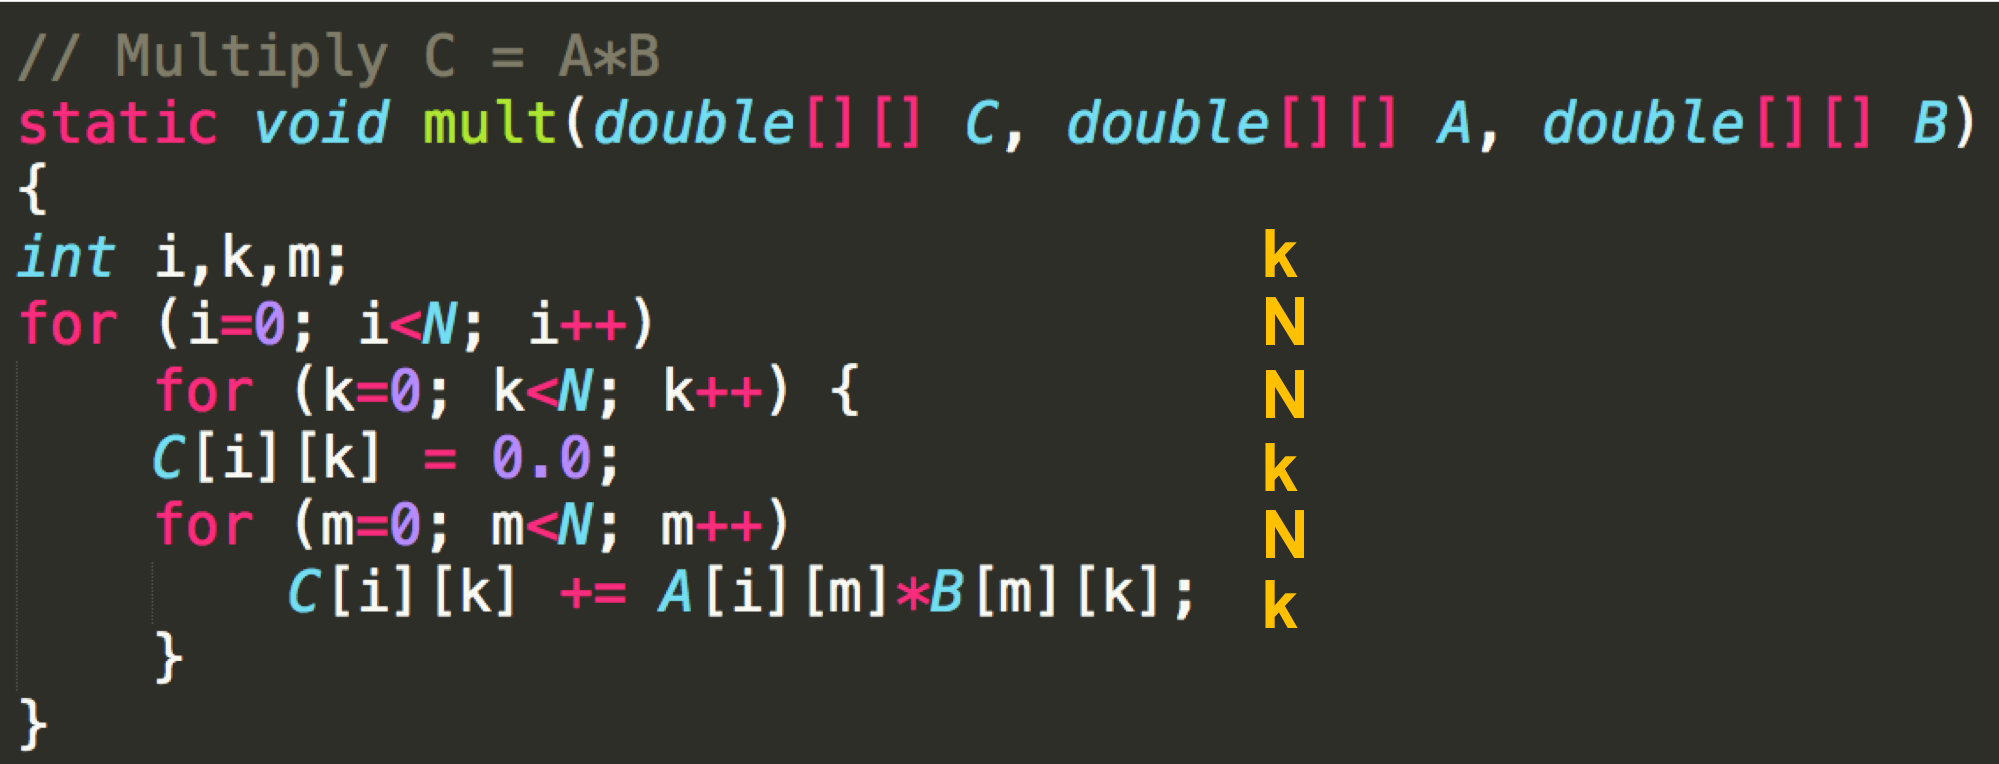
\includegraphics[width=.7\textwidth]{java.png}\\
\begin{align*}
	O(k + N\cdot (N + k+ N\cdot k))&=O(1+N\cdot(N+1+N\cdot 1))\\
	&=O(N\cdot(N+N))\\
	&=O(N\cdot(2\cdot N))\\
	&=O(N\cdot N)\\
	&=O(N^2)
\end{align*}
\\
C:\\\\
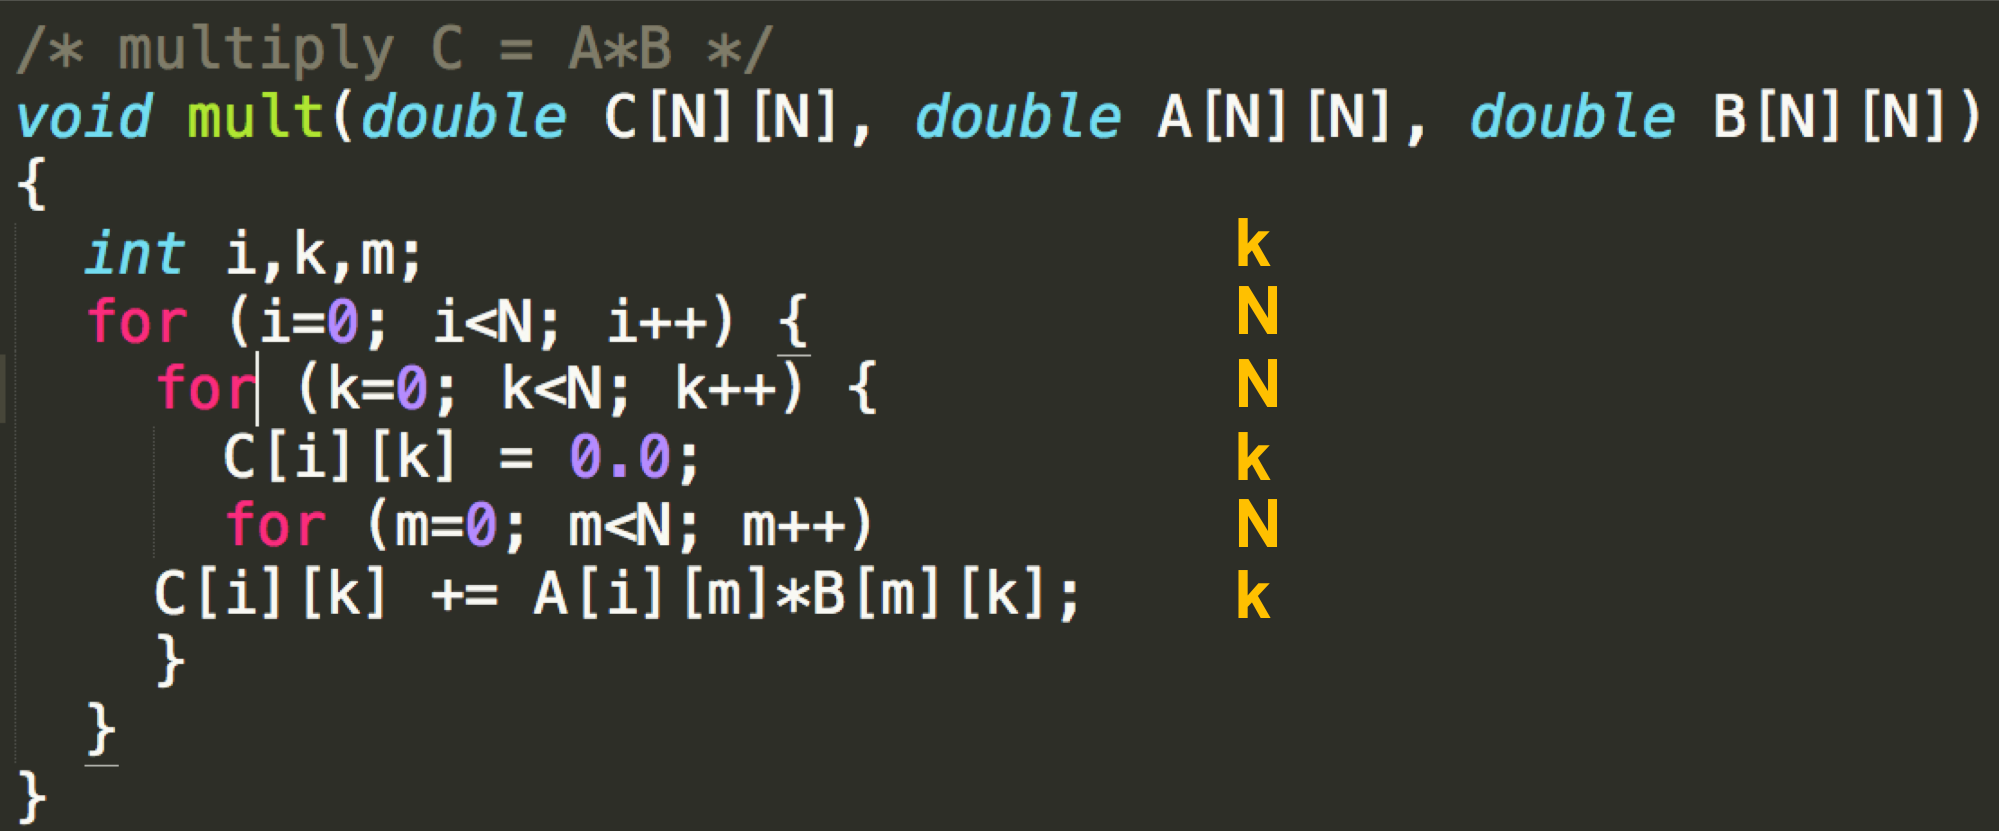
\includegraphics[width=.7\textwidth]{c.png}\\
\begin{align*}
O(k + N\cdot N\cdot(k + N\cdot k))&=O(1 + N\cdot N\cdot(1 + N\cdot 1))\\
&=O(N\cdot N\cdot N)\\
&=O(N^3)
\end{align*}
\\
Fazit:\\\\
Bei der empirischen Analyse sind wir durch eine Einschätzung von Messfehlern auf die selben Ergebnisse gekommen.
\end{document}
